\documentclass[12pt]{article}

% Packages:
\usepackage{graphicx}
\usepackage[portuguese]{babel}
\usepackage[utf8]{inputenc}
\usepackage{setspace}
\usepackage{listings}
\usepackage{hyperref}
\usepackage{tocloft}
\usepackage{fancyhdr}
\usepackage{placeins}
\usepackage{subcaption}
\usepackage{subfiles}
\usepackage{outlines}
\usepackage{indentfirst}
\usepackage{amsmath}
\usepackage{enumerate}
\usepackage{subfiles}
\usepackage{color, colortbl, xcolor}
\usepackage{multicol}
%---

% Options:
\setstretch{1} % Espaçamento entre linhas
\usepackage[top=3cm, bottom=2cm, left=1.5cm, right=1.5cm]{geometry}
\PassOptionsToPackage{hyphens}{url}
\title{}
\date{}

% Code customization:
% Default fixed font does not support bold face
\DeclareFixedFont{\ttb}{T1}{txtt}{bx}{n}{10} % for bold
\DeclareFixedFont{\ttm}{T1}{txtt}{m}{n}{10}  % for normal

\lstset{
	basicstyle=\footnotesize,
	columns=fullflexible,
    keywordstyle=\ttb\color{blue},
	stringstyle=\ttm\color{green},
	commentstyle=\color{gray},
	frame=None,
	breaklines=true,
	showstringspaces=false,
	postbreak=\mbox{\textcolor{red}{$\hookrightarrow$}\space},
}

%---
% Document:
\begin{document}
	% Cabeçalho:
\begin{figure}
		\begin{minipage}{.3\linewidth}
			\centering
			
\includegraphics[width=.6\linewidth]{imgs/ufpa.jpg}
		\end{minipage}
		\begin{minipage}{.70\linewidth}
			\flushleft
			\paragraph{}
			\textbf{ }\newline
			\textbf{UNIVERSIDADE FEDERAL DO PARÁ} \newline
			\textbf{INSTITUTO DE TECNOLOGIA} \newline
			\textbf{FACULDADE DE ENGENHARIA DA COMPUTAÇÃO E TELECOMUNICAÇÕES} \newline
			\textbf{TE05205 - Top. Especiais em Engenharia de Computação II} \newline
            \textbf{Prof. Dr. Roberto Celio Limão de Oliveira} \newline
            \textbf{Aluna: Camila Novaes Silva (201606840055)}
		\end{minipage}
\end{figure}
\FloatBarrier
\begin{center}
    {\Large \textbf{Atividade 06 - Medidas de diversidade}}
\end{center}
%%%%%%%%%%%%%
\hfill

Para calcular a medida de diversidade de uma população, utilizamos os algoritimos a seguir:

\begin{itemize}
	\item Medida de diversidade no fenótipo (MDF).\\
		Definida:
		\begin{equation}
			MDF = \frac{Fitness\ media\ da\ populacao}{Fitness\ do\ melhor\ individuo}
		\end{equation}
	\item Distância de Hamming.
\end{itemize}

A função a ser maximizada é
$$f6(x,y) = 0.5 - \frac{[\sin(\sqrt{(x^2 + y^2)})]^2 - 0.5}{[1 + 0.001(x^2 + y^2)]^2}$$.

% trim: left lower right upper

Assim, o objetivo é encontrar o valor de $x$,$y \in [-100,100]$ que maximiza a função $f$.

O AG utilizado foi o seguinte:

\begin{enumerate}[(a)]
	\item Representação binária: Para representar todos os valores dentro do intervalo $[-100,100]$, com uma precisão
		de 5 casa decimais foram necessários 25 bits para cada variável, totalizando 50 bits para cada cromossomo.

	\item Seleção: Roleta proporcional ao fitness.

	\item Operadores genéticos: Para realizar o cruzamento, foi utilizado o algoritmo ponto de corte, com apenas um ponto,
		com uma taxa de cruzamento de 75\%. E para a mutação foi utilizada uma taxa igual a 1\%.
	\item Critério de paragem: O critério de paragem foi 100 gerações.
\end{enumerate}

Os resultados obtidos são apresentados a seguir.

\begin{figure}[htb]
	\begin{subfigure}{.45\textwidth}
		\centering
		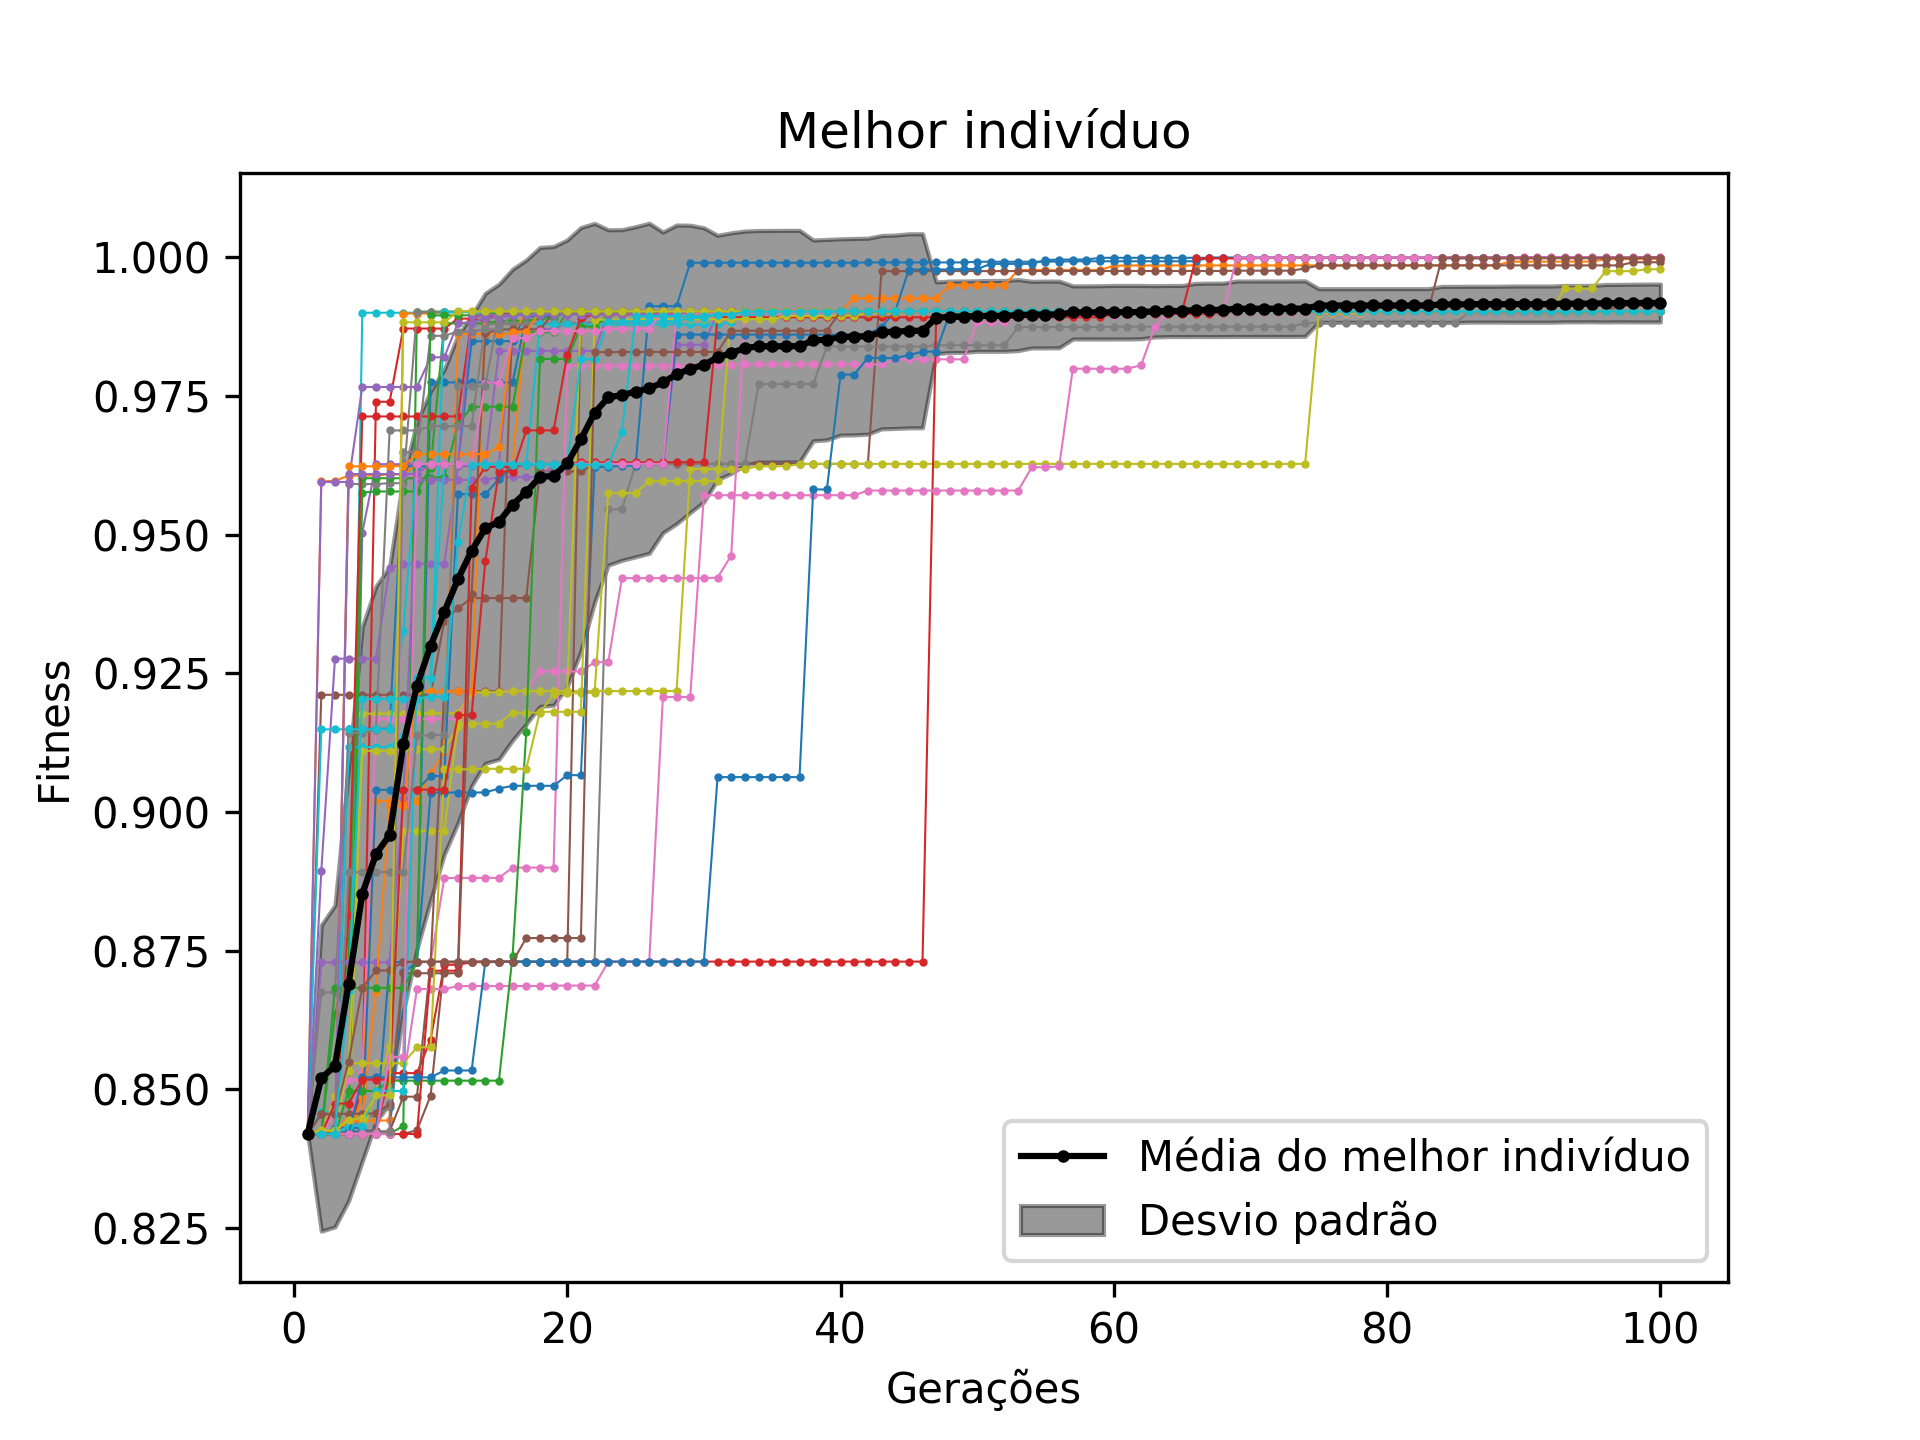
\includegraphics[width=1\textwidth]{./imgs/results/0_fitness_vs_gen_best.png}
		\caption{Melhores indíviduos de todos os experimentos ao longo das gerações.
		Em preto é mostrado o comportamento médio dos 50 experimentos. }
	\end{subfigure}
	\hfill
	\begin{subfigure}{.45\textwidth}
		\centering
		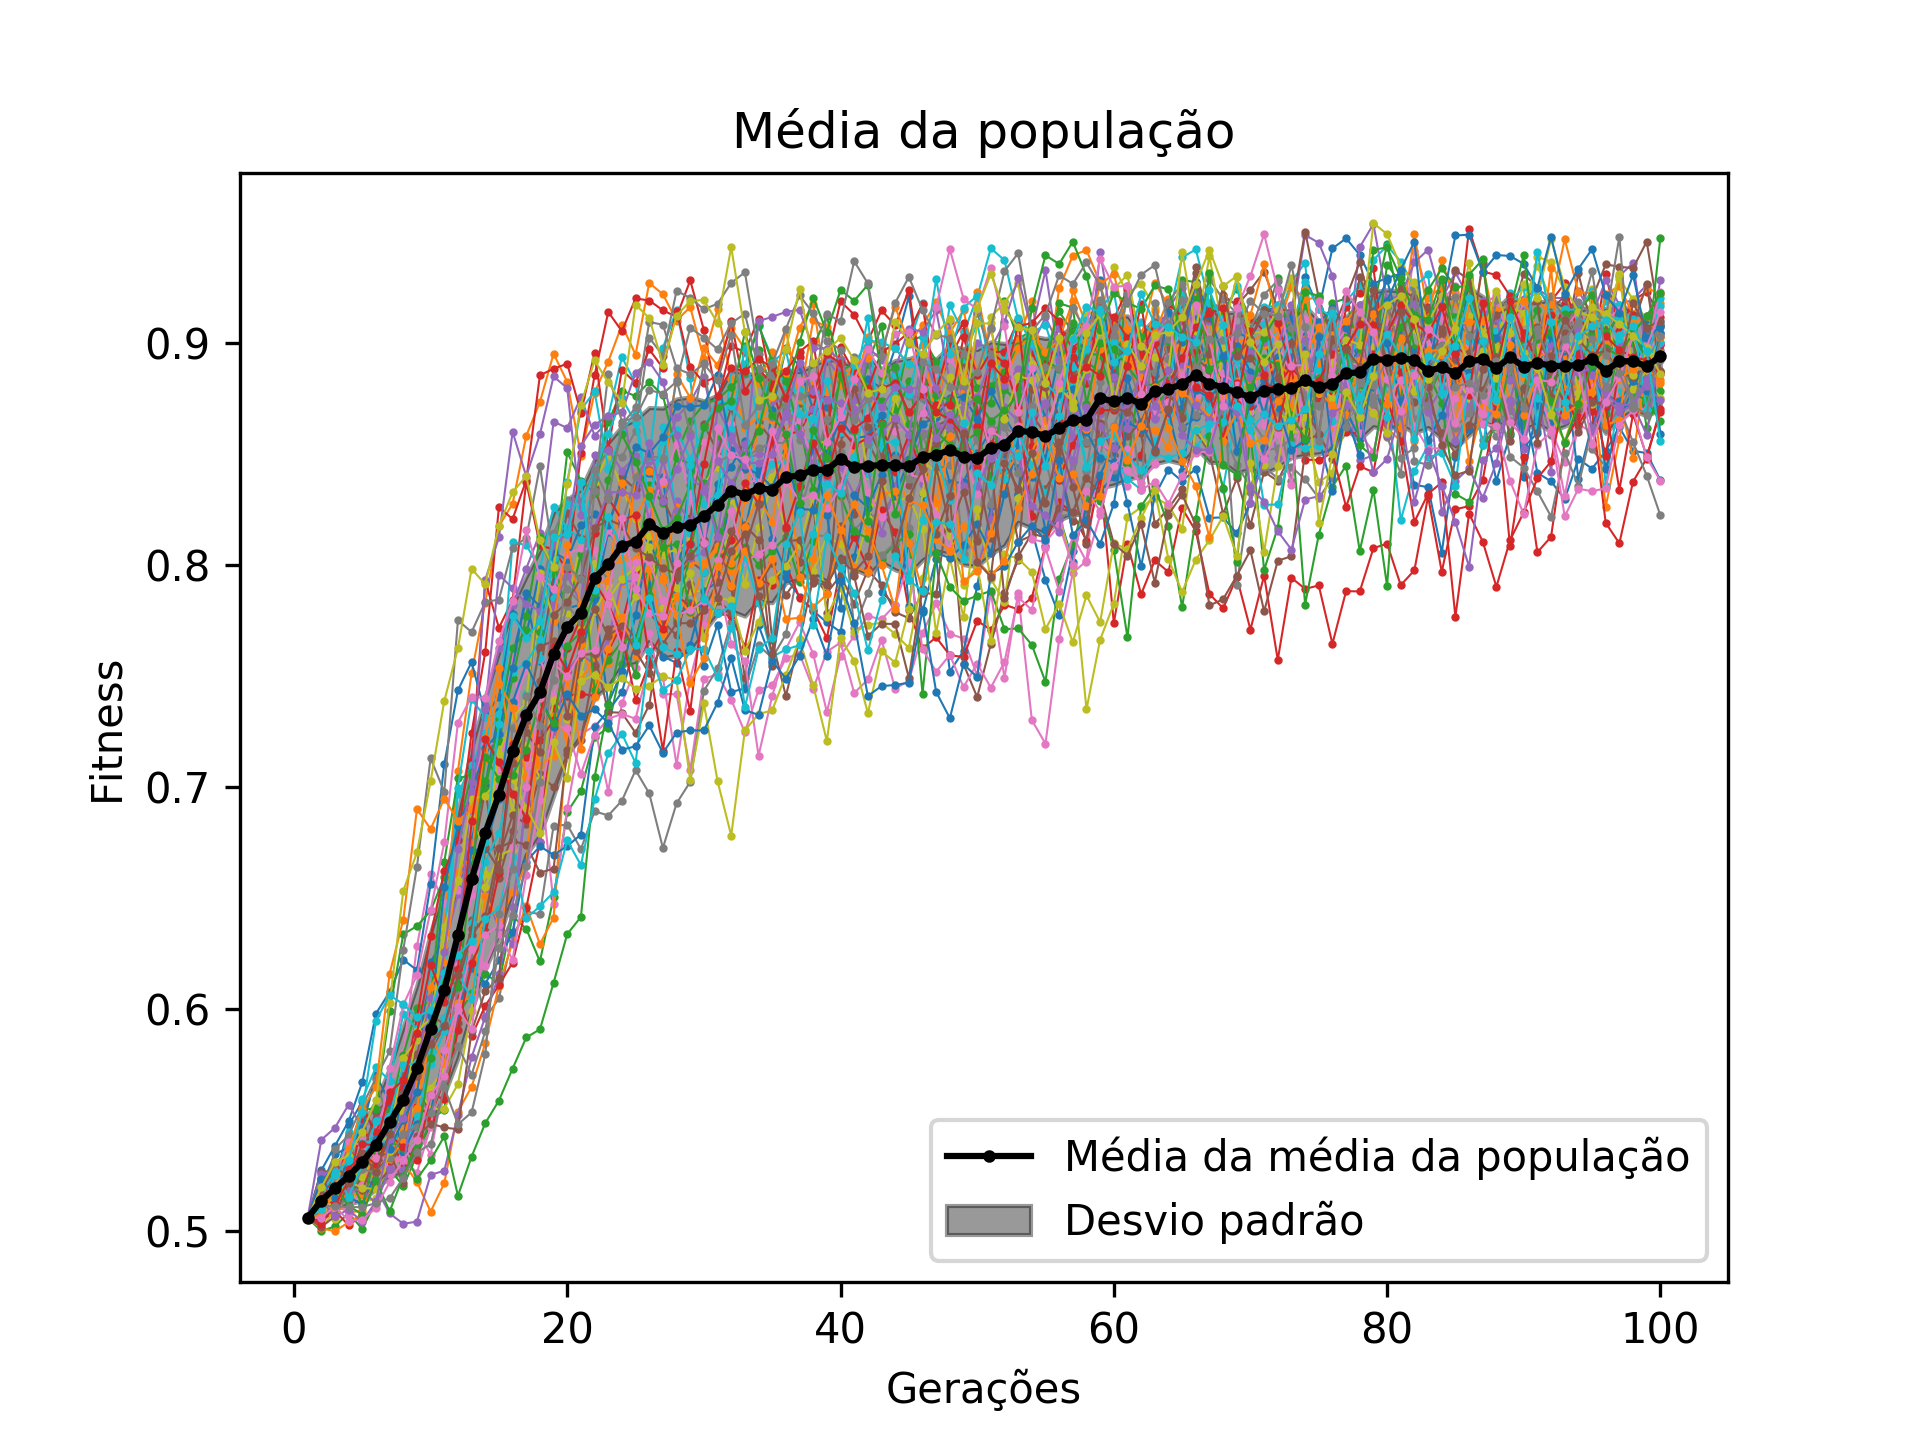
\includegraphics[width=1\textwidth]{./imgs/results/0_fitness_vs_gen_pop.png}
		\caption{Média da população de todos os experimentos ao longo das gerações.
		Em preto é mostrado o comportamento médio dos 50 experimentos.}
	\end{subfigure}
	\caption{Resultados obtidos no teste número 3 da tabela~\ref{tab:f6_prop}}
\end{figure}

\begin{figure}
	\centering
	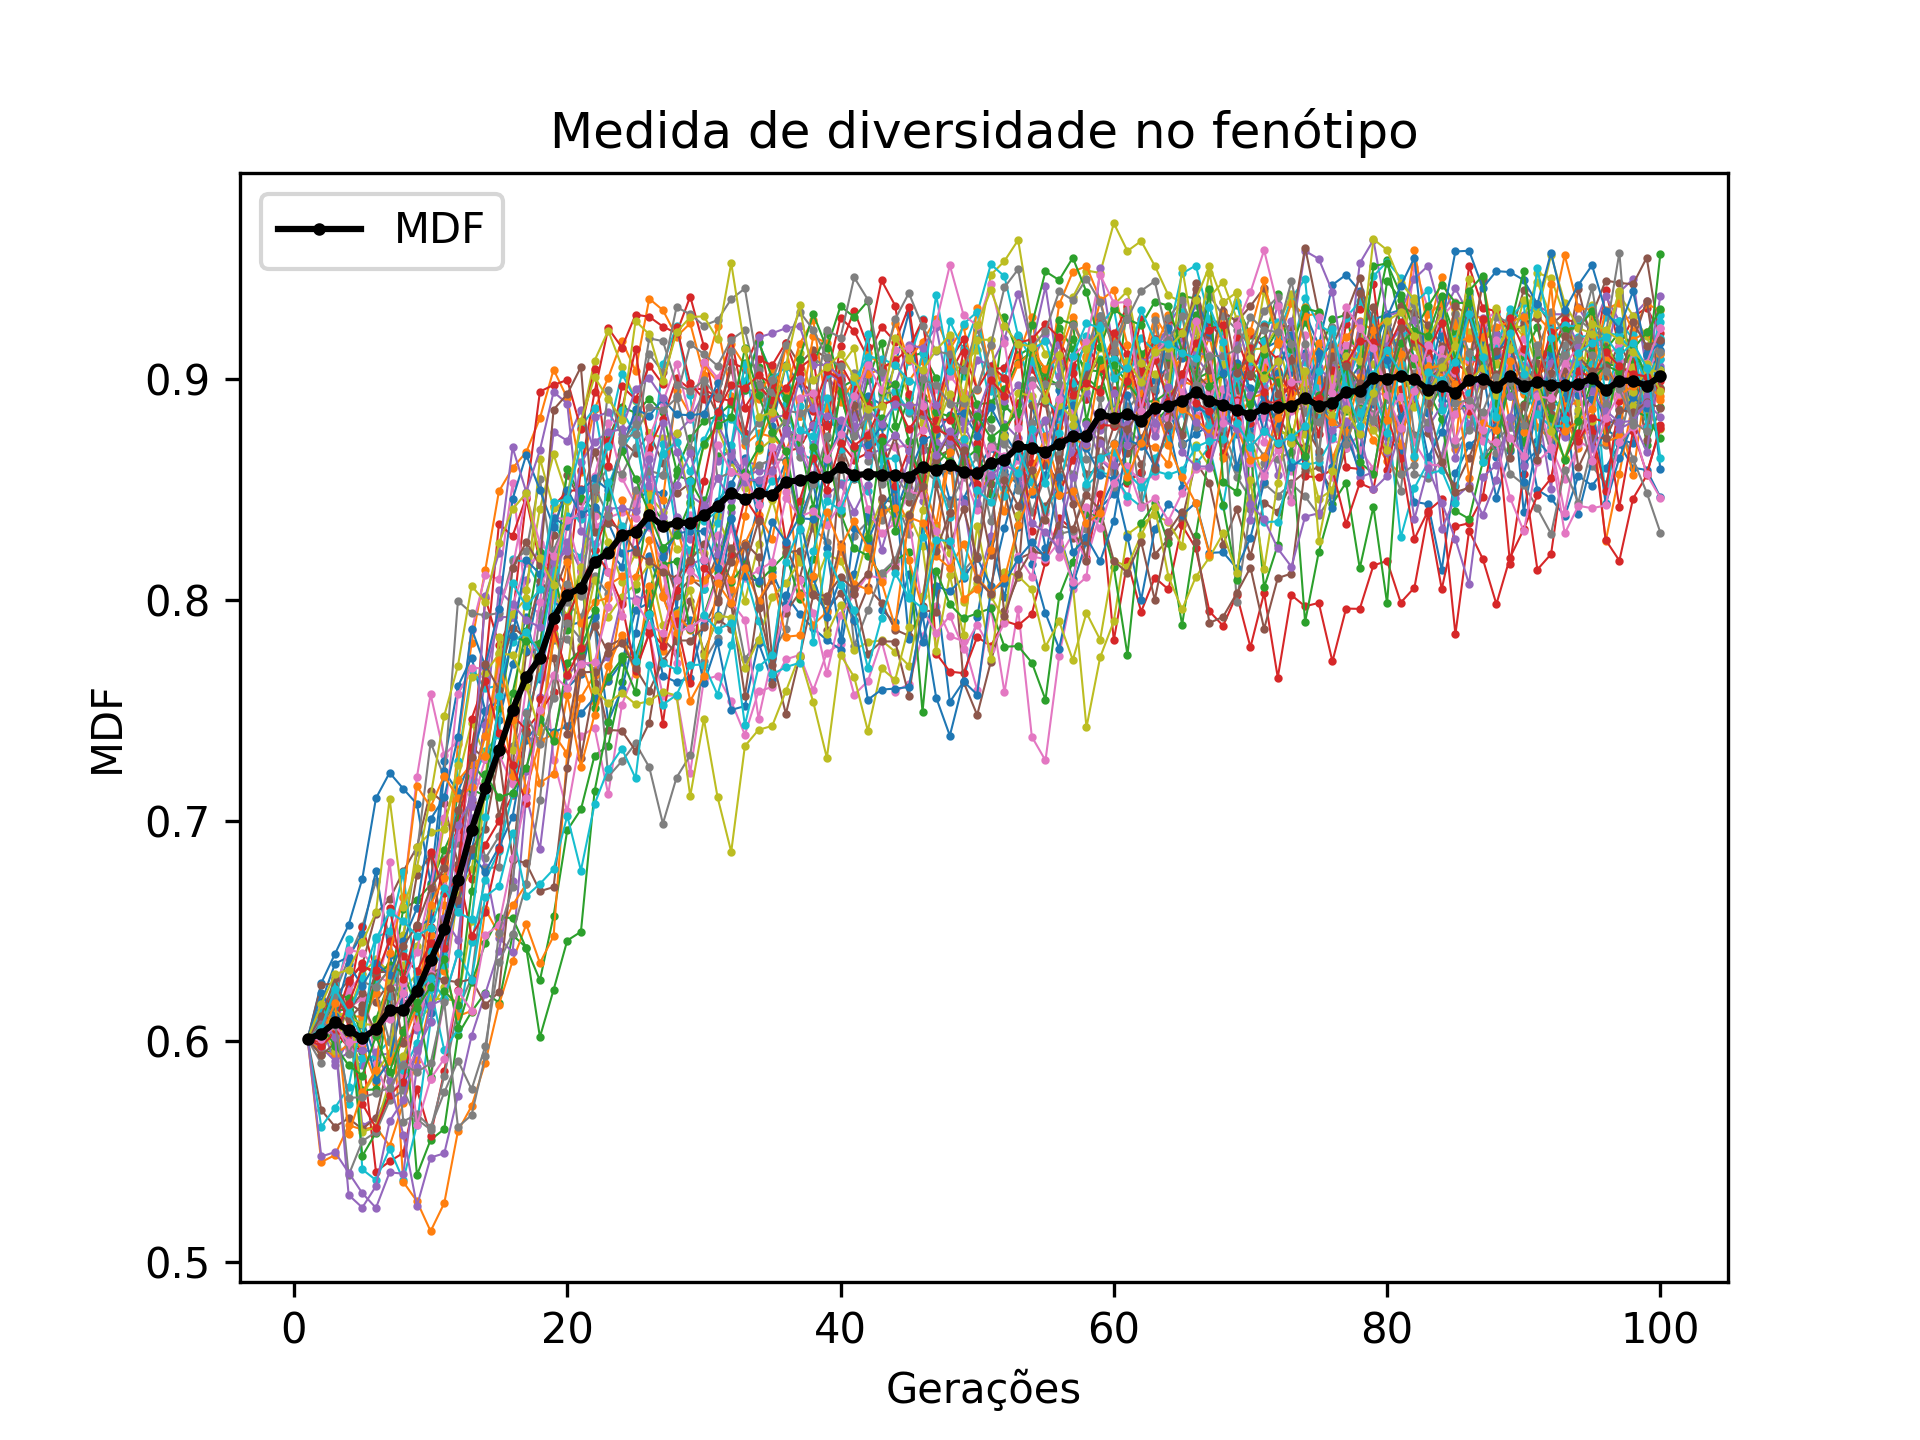
\includegraphics[width=1\textwidth]{imgs/results/0_fitness_vs_gen_mdf.png}
	\caption{Medida de diversidade no fenótipo. Em preto é representado a média dos 50 experimentos.}
\end{figure}

\begin{figure}
	\centering
	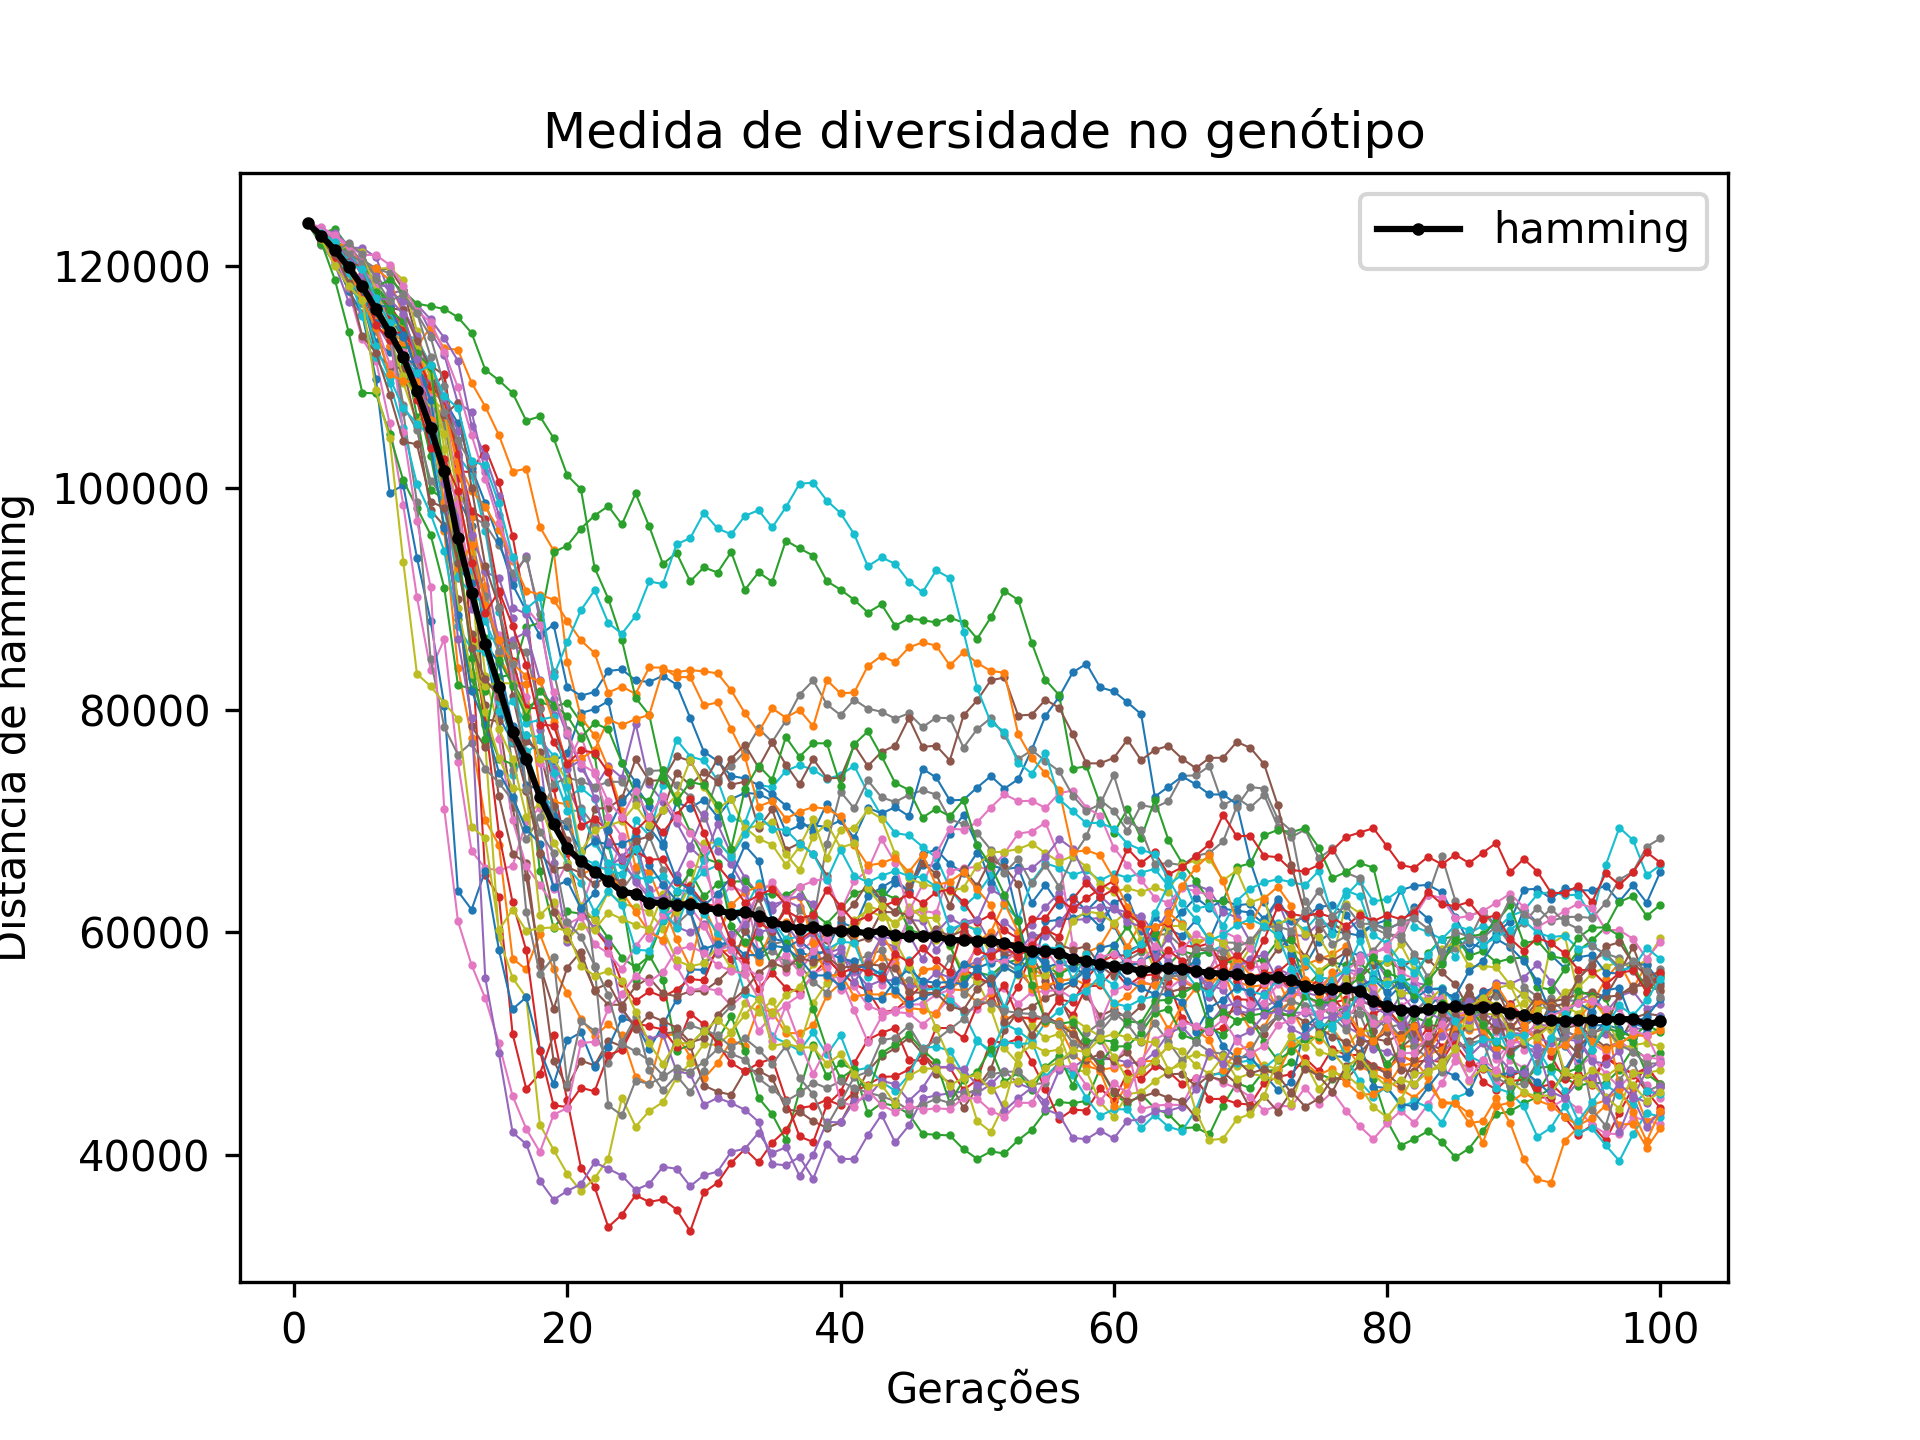
\includegraphics[width=1\textwidth]{imgs/results/0_fitness_vs_gen_hamming.png}
	\caption{Medida de diversidade no genótipo utilizando a distância de hamming. Em preto é representado a média dos 50 experimentos}
\end{figure}


	\begin{figure}[htb]
	\begin{subfigure}{.5\textwidth}
		\centering
		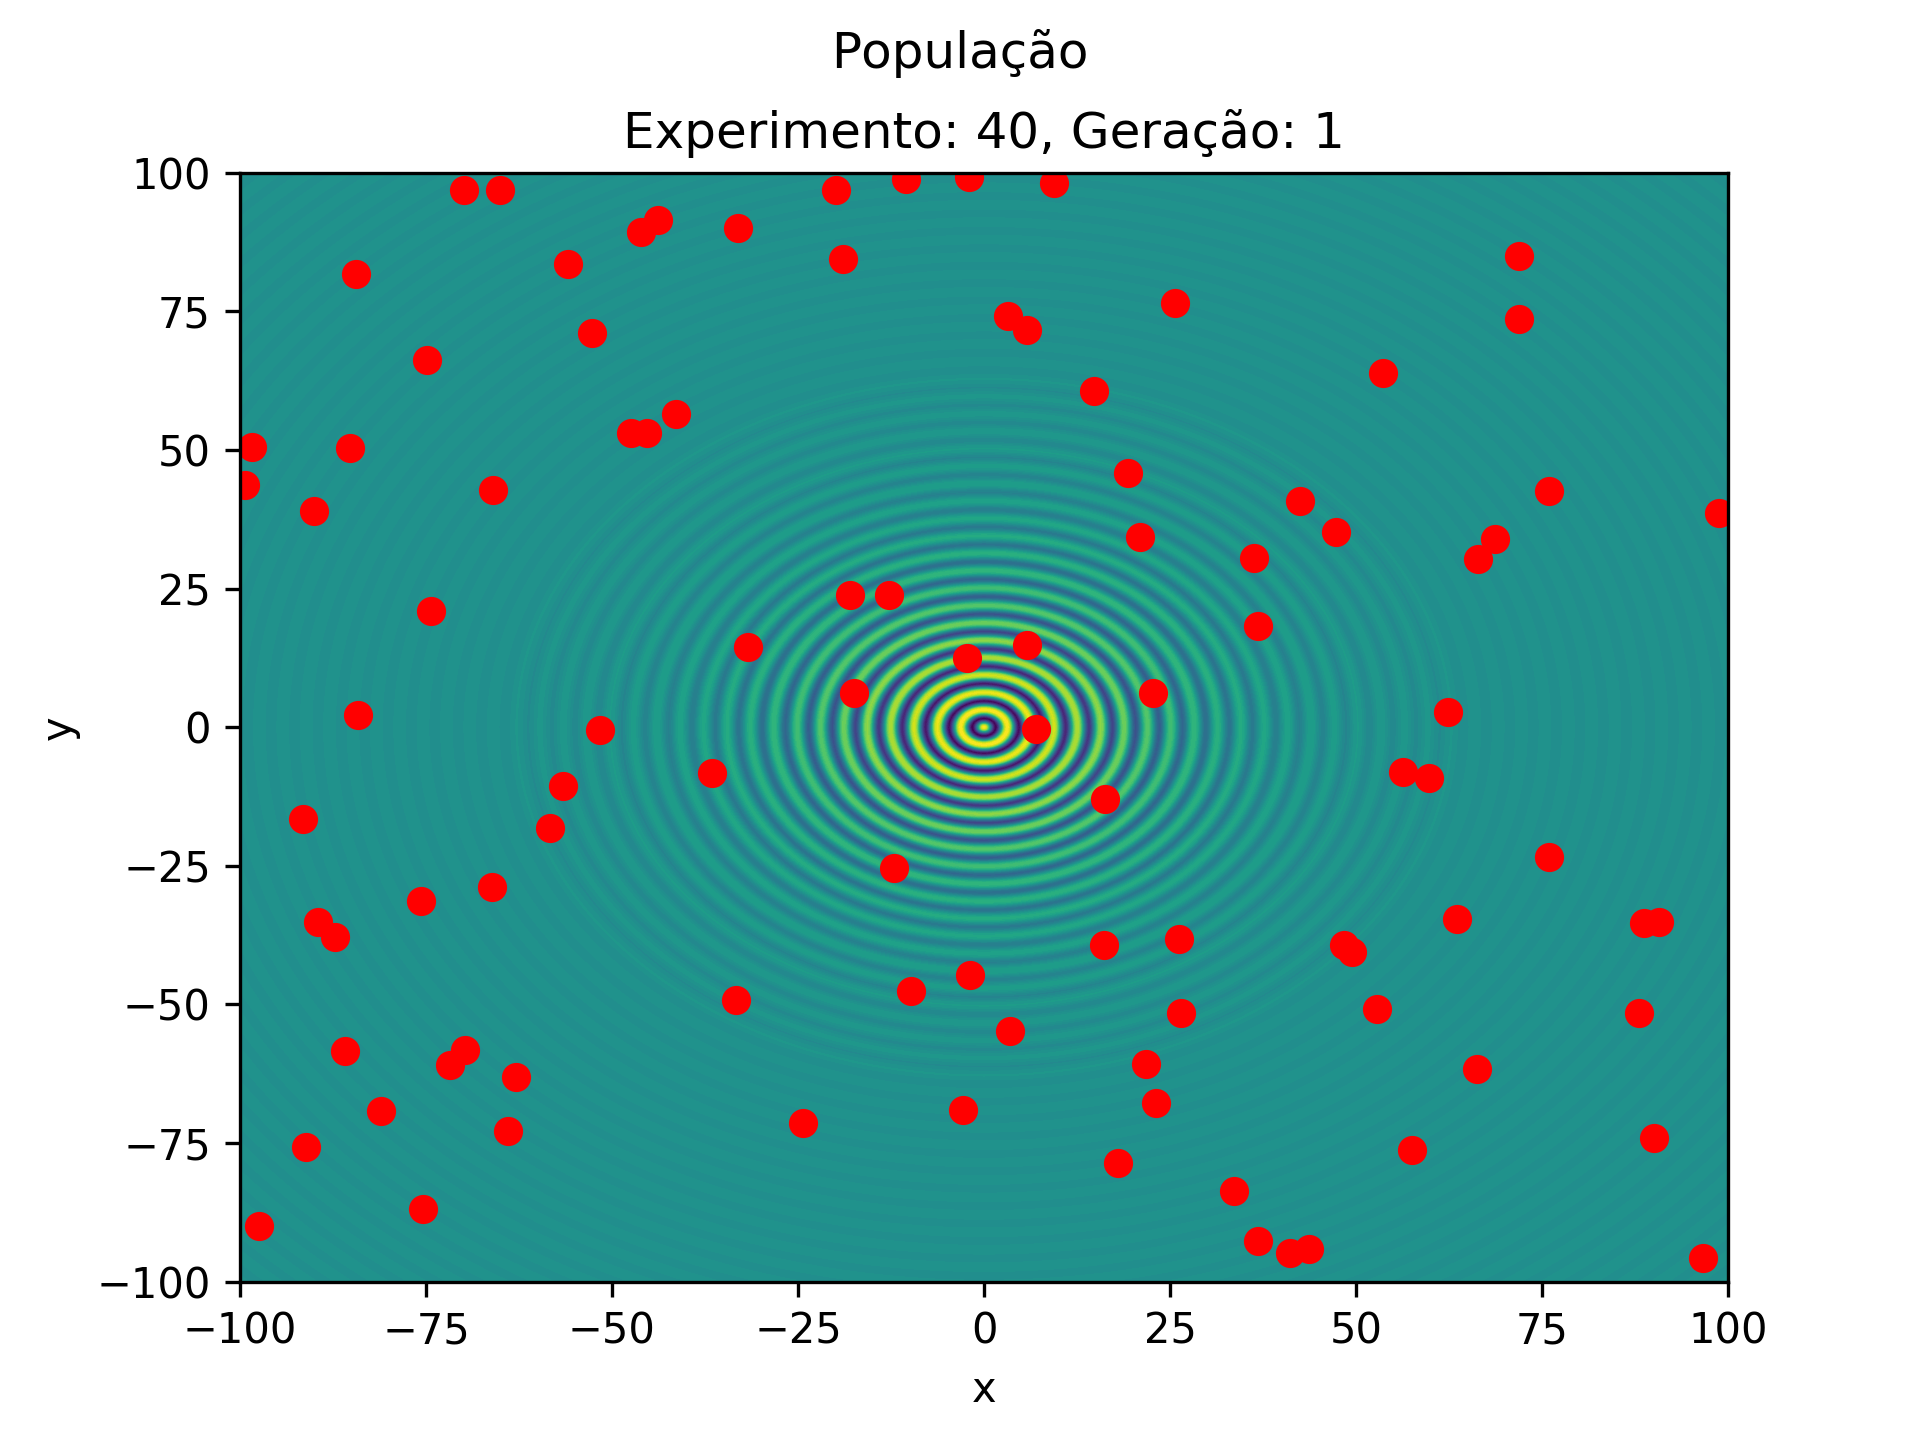
\includegraphics[width=0.9\linewidth]{./imgs/results/0_population_gen_1_exp_40.png}
	  \end{subfigure}
	  \begin{subfigure}{.5\textwidth}
		\centering
		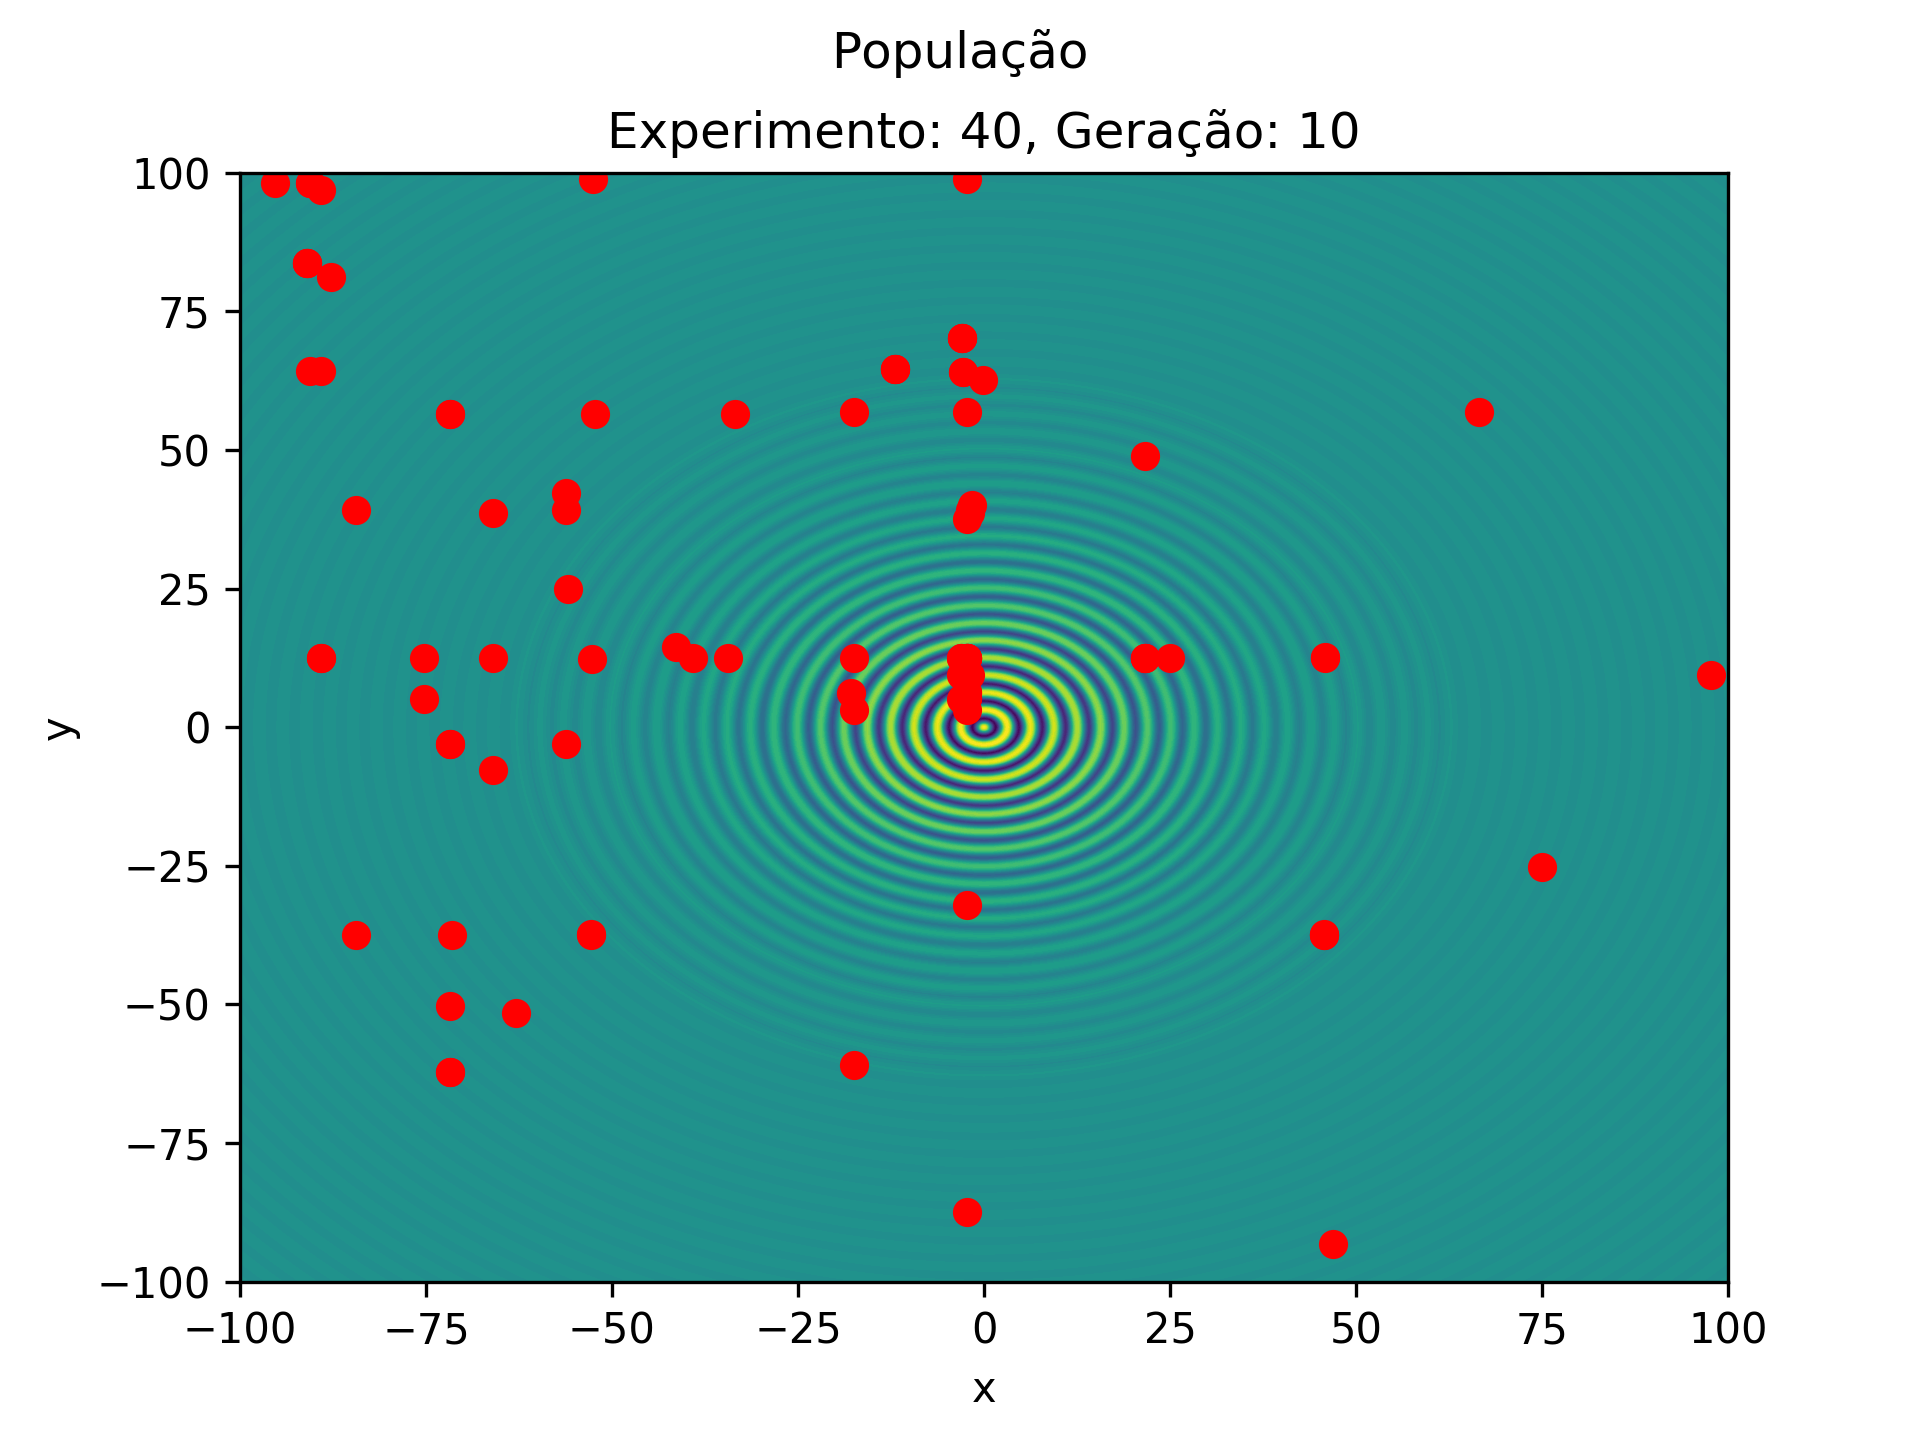
\includegraphics[width=0.9\linewidth]{./imgs/results/0_population_gen_10_exp_40.png}
	  \end{subfigure}
	  \begin{subfigure}{.5\textwidth}
		\centering
		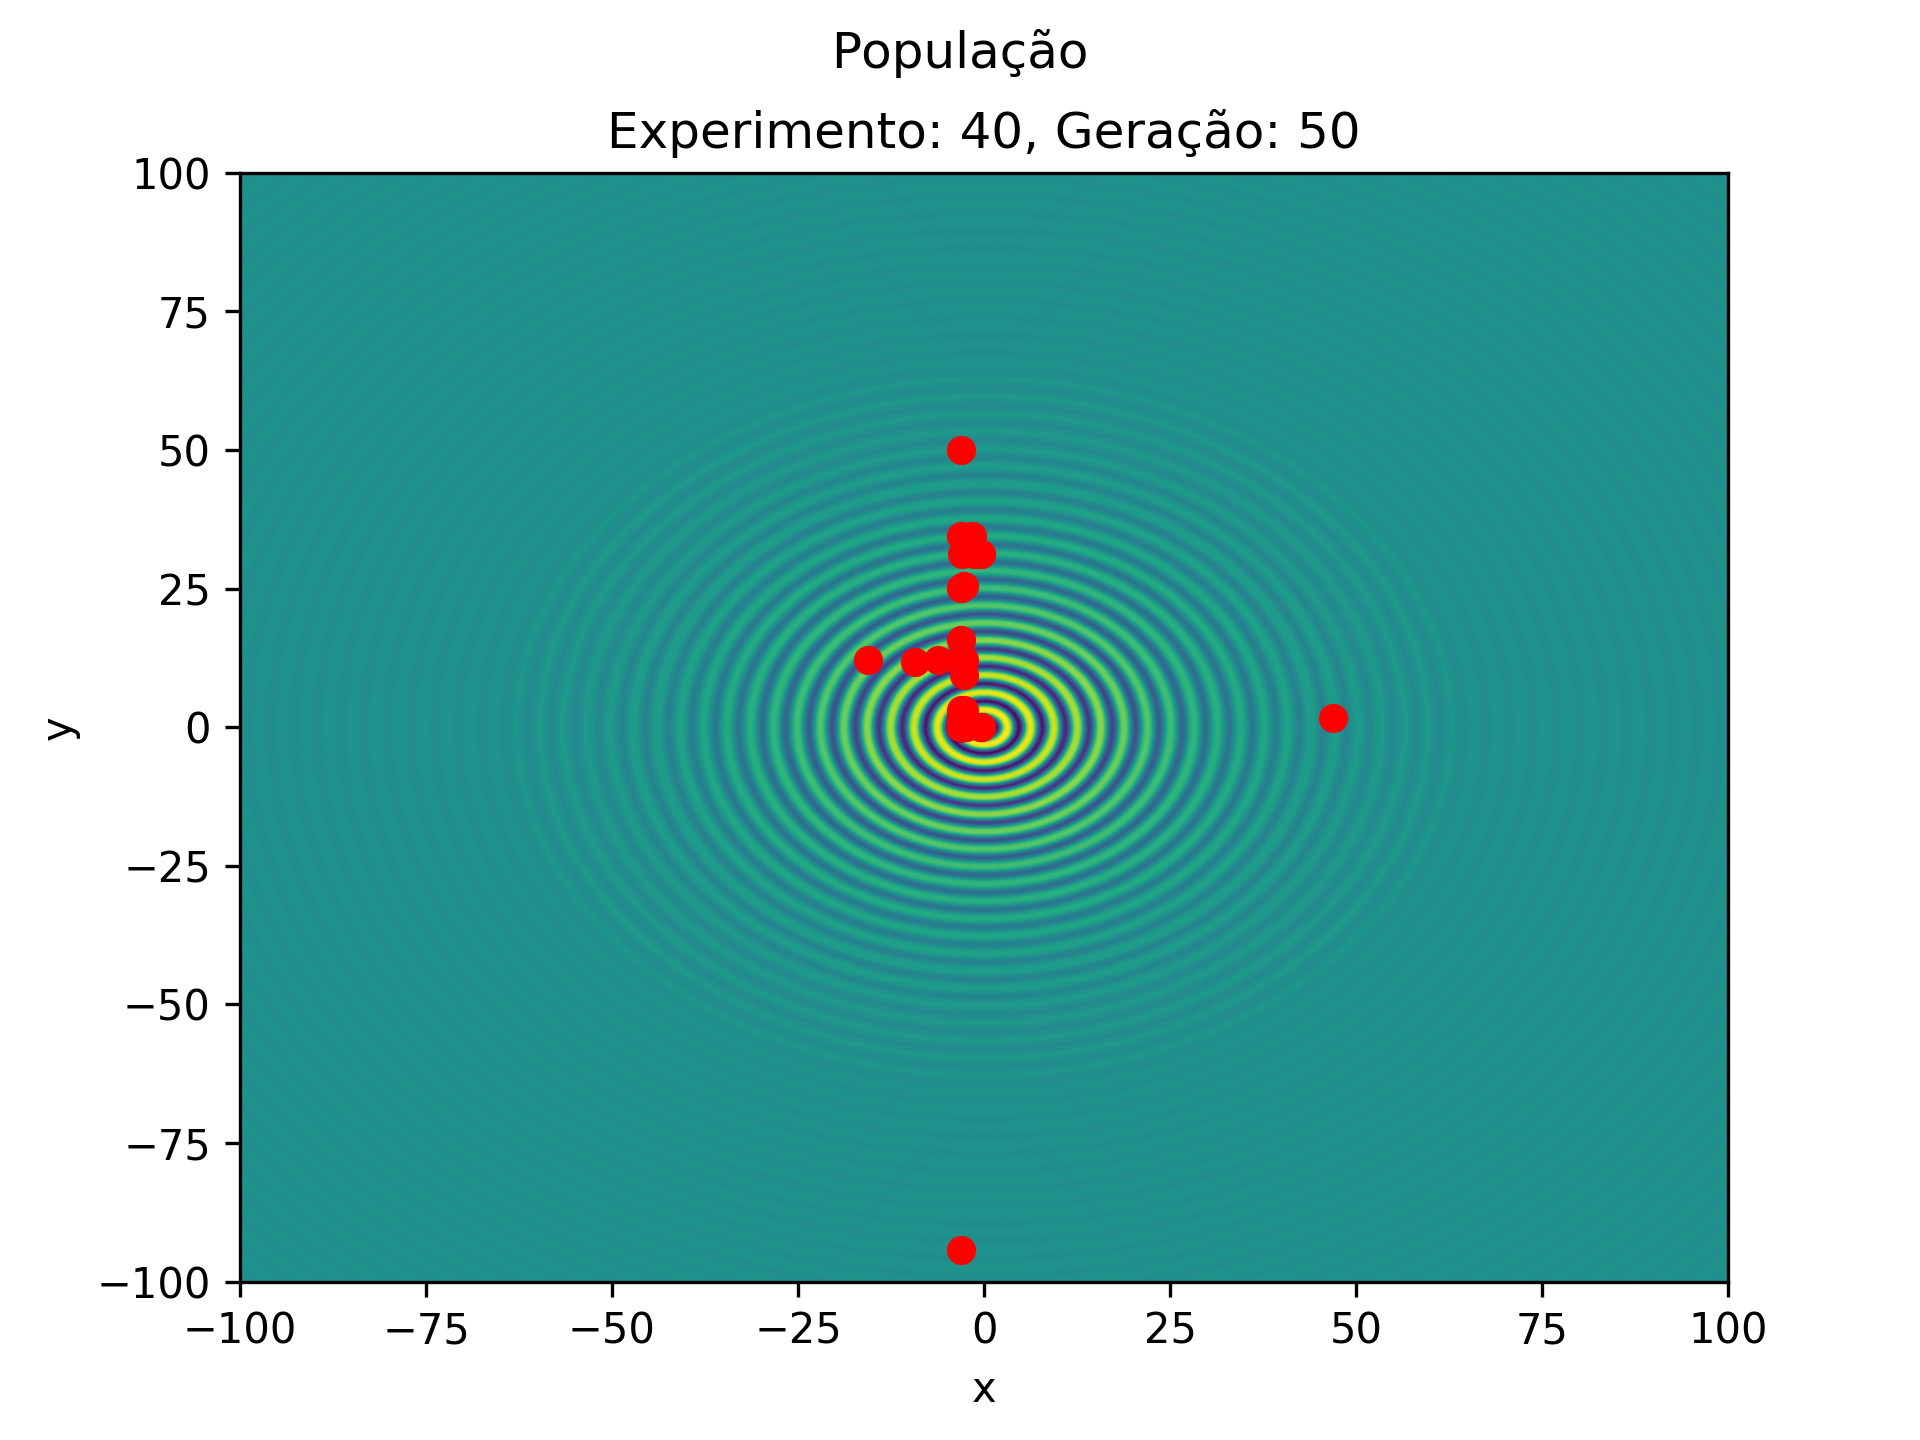
\includegraphics[width=0.9\linewidth]{./imgs/results/0_population_gen_50_exp_40.png}
	  \end{subfigure}
	  \begin{subfigure}{.5\textwidth}
		\centering
		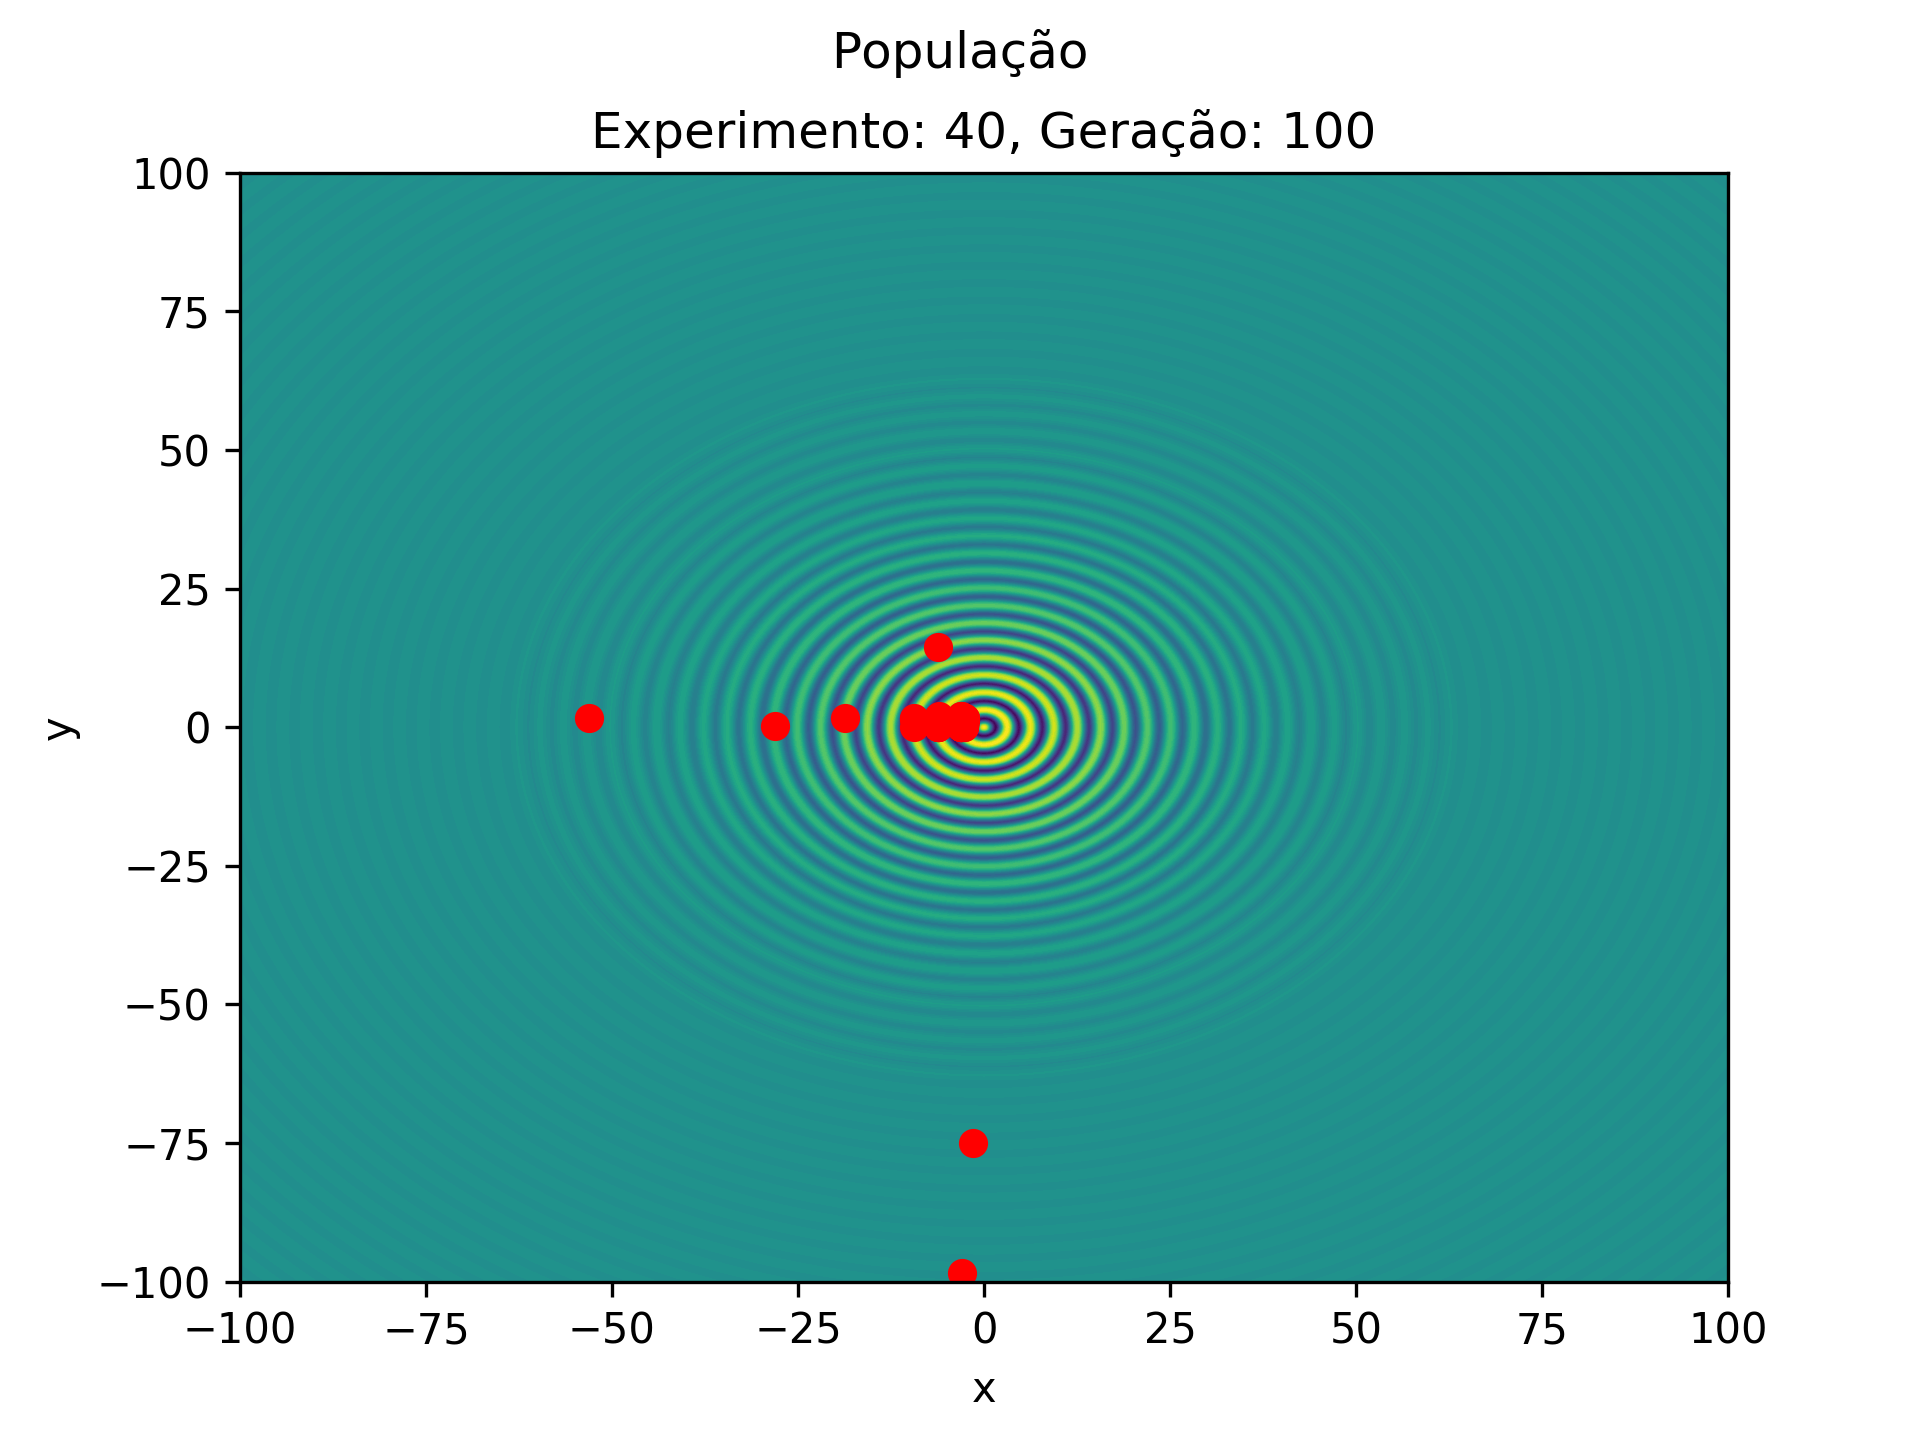
\includegraphics[width=0.9\linewidth]{./imgs/results/0_population_gen_100_exp_40.png}
	  \end{subfigure}
	\caption{Populações do experimento 40 nas gerações 1, 10, 50 e 100.}
	\end{figure}
\end{document}
